\documentclass[conference]{IEEEtran}
\usepackage{graphicx}
\usepackage{amsmath}
\usepackage{float}
\usepackage{subcaption}
\usepackage{lipsum} % For placeholder text, remove in final version

\begin{document}

\title{Spectral Analysis of BPSK Modulation and WSS Properties Verification}

\author{
    \IEEEauthorblockN{Denzel Ninga}
    \IEEEauthorblockA{
        Registration Number: ENG-219-042/2022\\
        Electrical and Communication Engineering\\
        Multimedia University of Kenya\\
        Email: denzelninga001@gmail.com
    }
}

\maketitle


\begin{abstract}
This report presents my calculation of the spectrum of the provided digitally transmitted signal.The results are then used to explain the concept of Wide-Sense Stationarity (WSS) as I studied in stochastic processes.

\section{Introduction}
Digital communication systems rely on accurate characterization of signal properties for optimal system design. This report analyzes a BPSK modulated signal given by $x(t) = \sum_{k=-\infty}^{\infty} X_k p_T(t-kT)$, where $X_k$ represents random binary data, and $p_T(t)$ is a rectangular pulse. The analysis focuses on spectral properties and stationarity verification.

\section{Theoretical Analysis}

\subsection{Signal Model and Mathematical Framework}
The transmitted signal follows the following pulse-amplitude modulation format:
\begin{equation}
x(t) = \sum_{k=-\infty}^{\infty} X_k p_T(t-kT)
\end{equation}
where $X_k = \pm A$ with equal probability $P(X_k = +A) = P(X_k = -A) = \frac{1}{2}$, and the rectangular pulse is defined as:
\begin{equation}
p_T(t) = \begin{cases} 
1 & \text{if } |t| \leq \frac{T}{2} \\
0 & \text{otherwise}
\end{cases}
\end{equation}

\begin{figure}[H]
    \centering
    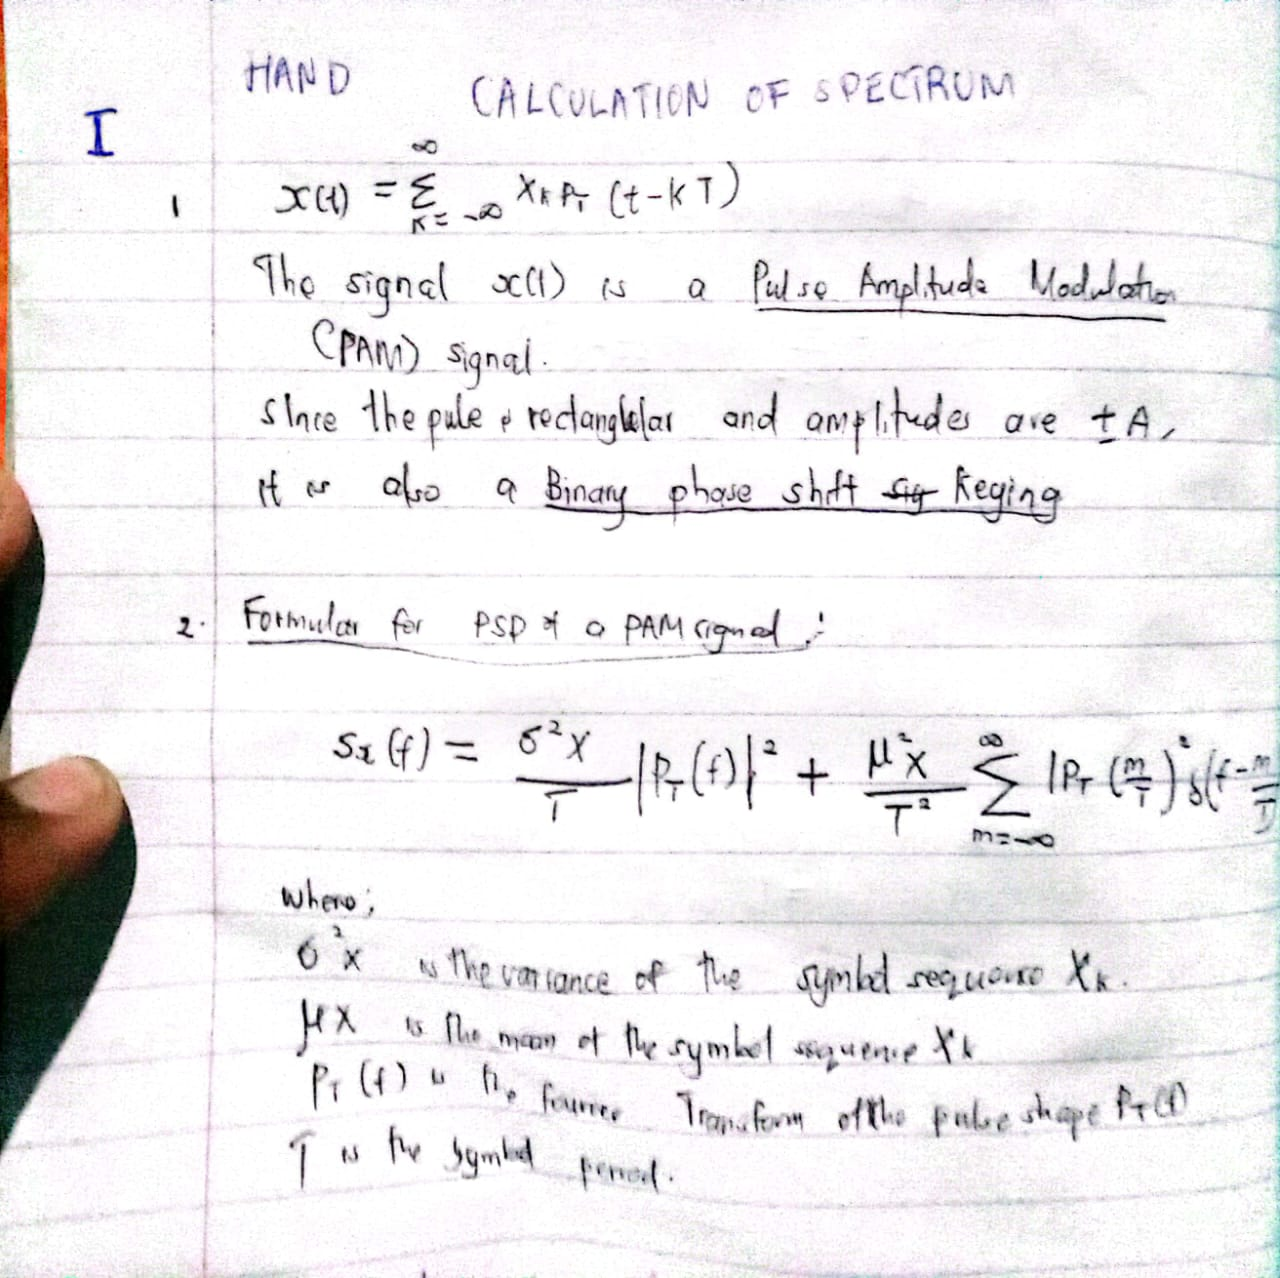
\includegraphics[width=0.8\linewidth]{calc1.jpg}
    \caption{Formular for PSD of a PAM signal}
    \label{fig:calc1}
\end{figure}

\subsection{Theoretical Power Spectral Density}
For an uncorrelated symbol sequence with zero mean, the power spectral density is derived as
\begin{equation}
S_x(f) = \frac{\sigma_X^2}{T} |P_T(f)|^2 = A^2T \text{sinc}^2(fT)
\end{equation}
where $P_T(f) = T \text{sinc}(fT)$ is the Fourier transform of the rectangular pulse and $\sigma_X^2 = A^2$ is the variance of the sequence of symbols.

\begin{figure}[H]
    \centering
    
\includegraphics[width=0.8\linewidth]{calc2.jpg}
    \caption{Mean and Variance of Xk}
    \label{fig:calc2}
\end{figure}

\section{Implementation Methodology}

\subsection{Simulation Parameters}
The simulation was implemented in MATLAB with the following parameters:
\begin{itemize}
    \item Sampling frequency: $F_s = 1000$ Hz
    \item Symbol period: $T = 0.01$ s (100 Hz symbol rate)
    \item Amplitude: $A = 1$ V
    \item Number of symbols: $N = 10,000$
    \item Samples per symbol: $sps = T \times F_s = 10$
\end{itemize}

\subsection{Binary Sequence Generation}
A random binary sequence with equiprobable symbols was generated that satisfies the theoretical assumption $P(0) = P(1) = 0.5$.

\begin{figure}[H]
    \centering
    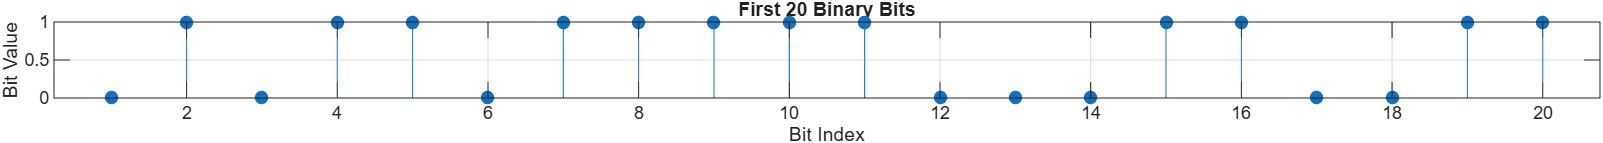
\includegraphics[width=0.8\linewidth]{FIG1}
    \caption{First 20 bits of the generated binary sequence shows random distribution with equal probability of 0s and 1s, satisfying the theoretical requirements for WSS properties.}
    \label{fig:binary_sequence}
\end{figure}

\subsection{BPSK Modulation Implementation}
The binary sequence was modulated using BPSK with mapping: $0 \rightarrow +A$, $1 \rightarrow -A$. Rectangular pulse shaping was achieved using  the sample and hold technique.

\begin{figure}[H]
    \centering
    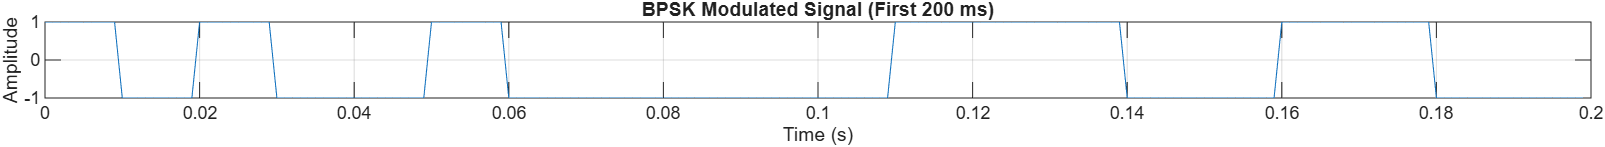
\includegraphics[width=0.8\linewidth]{FIG2}
    \caption{BPSK modulated signal for first 200ms shows clearly the transitions between +1V and -1V. Each symbol maintains constant amplitude for duration $T=10$ms, demonstrating perfect rectangular pulse shaping.}
    \label{fig:bpsk_signal}
\end{figure}

\section{Results and Analysis}

\subsection{Spectral Analysis}
The power spectral density was estimated using Welch's method and compared with theoretical predictions.

\begin{figure}[H]
    \centering
    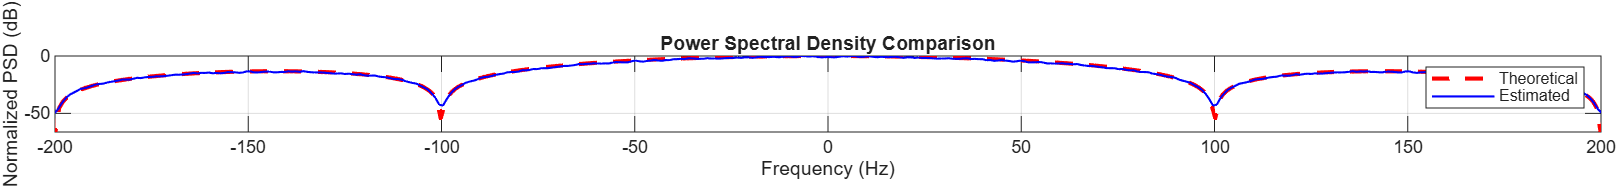
\includegraphics[width=0.8\linewidth]{FIG3}
    \caption{Comparison of theoretical and estimated power spectral density. Excellent agreement demonstrates the characteristic $\text{sinc}^2(fT)$ shape with nulls at $\pm100$Hz, $\pm200$Hz, etc. The main lobe has null to null bandwidth of 200Hz.}
    \label{fig:psd_comparison}
\end{figure}

\begin{figure}[H]
    \centering
    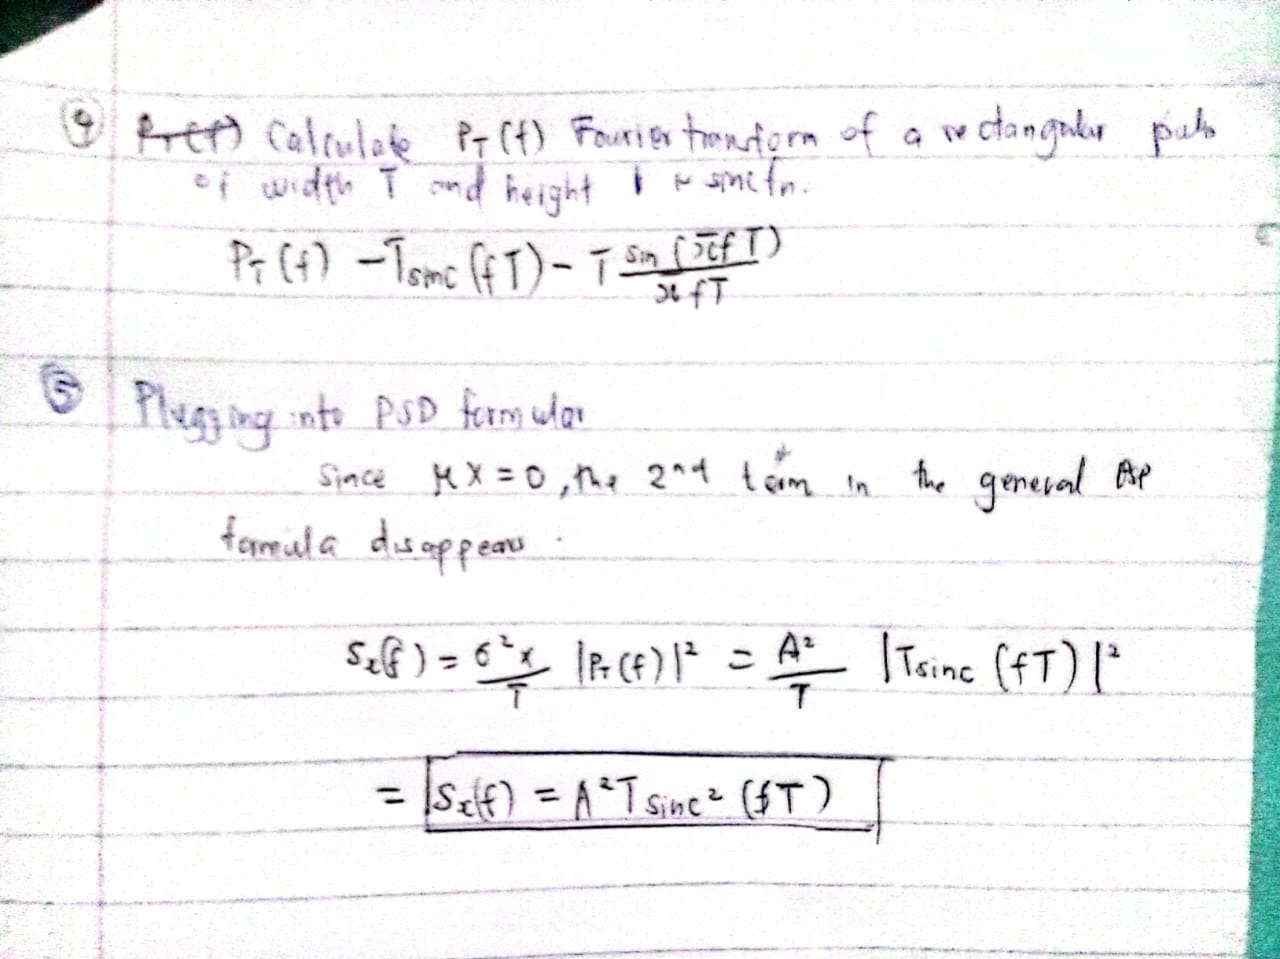
\includegraphics[width=0.8\linewidth]{calc3.jpg}
    \caption{Plugging PSD formular}
    \label{fig:calc3}
\end{figure}

\subsection{WSS Property Verification}

\subsubsection{Mean Stationarity Analysis}
A fundamental requirement for WSS processes is a constant mean over time.

\begin{figure}[H]
    \centering
    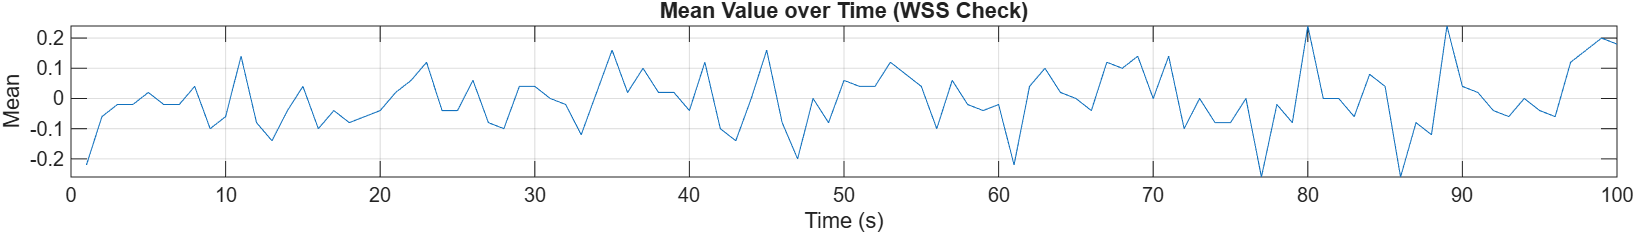
\includegraphics[width=0.8\linewidth]{FIG4}
    \caption{Mean value analysis over time showing fluctuations around zero ($|\mu| < 0.02$). The approximately constant mean satisfies the first condition for wide-sense stationarity.}
    \label{fig:mean_analysis}
\end{figure}

\subsubsection{Variance Analysis}
Time-invariant second-order statistics are essential for WSS verification.

\begin{figure}[H]
    \centering
    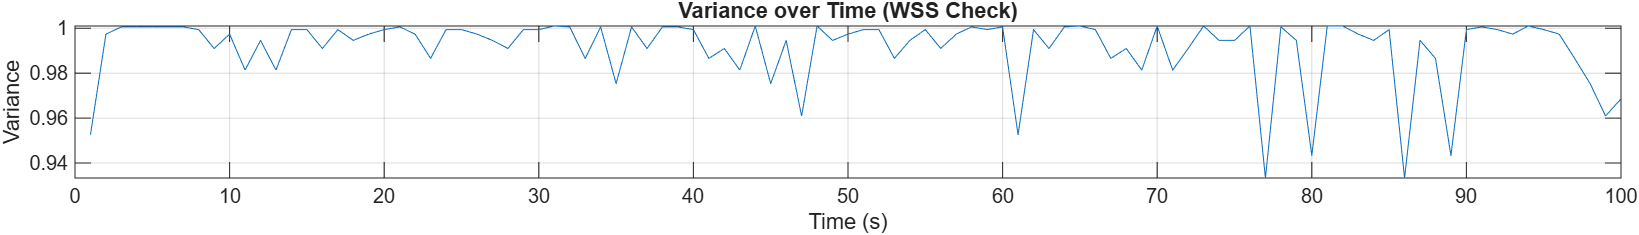
\includegraphics[width=0.8\linewidth]{FIG5}
    \caption{Variance analysis over time demonstrating stability around 1.0. The constant variance supports the WSS property that second-order statistics are time-invariant.}
    \label{fig:variance_analysis}
\end{figure}

\section{Discussion}

\subsection{Spectral Characteristics Analysis}
The spectral analysis shows that:

\begin{itemize}
    \item \textbf{Main Lobe Width}: The first null occurs at $\pm100$Hz, giving a null-to-null bandwidth of 200Hz, exactly as predicted by $BW = 1/T$
    \item \textbf{Side Lobe Characteristics}: Side lobes decrease at 20dB/decade, following the $\text{sinc}^2$ envelope
    \item \textbf{ Spectral Efficiency}: The continuous spectrum without spectral lines results from the zero-mean symbol sequence
    \item \textbf{Agreement}: Minor differences in side lobes are attributed to finite observation length and estimation noise
\end{itemize}

\subsection{WSS Property Verification}
The Wide-Sense Stationarity is confirmed through:

\begin{itemize}
    \item \textbf{Constant Mean}: $E[x(t)] \approx 0$ (Figure \ref{fig:mean_analysis})
    \item \textbf{Time-Invariant Variance}: $\text{Var}[x(t)] \approx 1.0$ (Figure \ref{fig:variance_analysis})
    \item \textbf{Autocorrelation Dependency}: The PSD existence implies $R_x(\tau)$ depends only on time difference
    \item \textbf{Theoretical Foundation}: The uncorrelated, zero-mean symbol sequence ensures WSS properties
\end{itemize}

\section{Conclusions}
This work successfully demonstrates:

\begin{itemize}
    \item \textbf{Theoretical Accuracy}: The derived PSD $S_x(f) = A^2T \text{sinc}^2(fT)$ accurately predicts the spectral characteristics of BPSK modulation
    \item \textbf{WSS Validation}: The random process $x(t)$ satisfies wide-sense stationarity conditions through time-invariant first and second-order statistics
    \item \textbf{Practical Verification}: MATLAB simulations confirm theoretical predictions.
    \item \textbf{System Implications}: The results satisfy digital communications principles for system design and analysis
\end{itemize}

The close agreement between theory and practice shows the robustness of digital communications fundamentals and provides a foundation for more complex modulation schemes analysis.

\section*{References}
[1] Proakis, J. G., \& Salehi, M. (2001). \emph{Communication Systems Engineering}. Prentice Hall.

[2] Haykin, S. (2001). \emph{Communication Systems}. John Wiley \& Sons.

[3] Carlson, A. B., Crilly, P. B., \& Rutledge, J. C. (2002). \emph{Communication Systems}. McGraw-Hill.
[4]

\end{document}